\label{Wireshark Packet Filtering}
\chapter{Wireshark Packet Filtering}
\section{Ping tool}
\begin{itemize}
\item Ping tool is utility used for troubleshooting, testing an diagnosing issues related to network connectivity 
\item When we use Wireshark for capturing live packets in the background we parallelly use terminal and ping www.google.com 
\item We let Wireshark to capture the packets for few seconds 
\begin{figure}[H]
\centering
  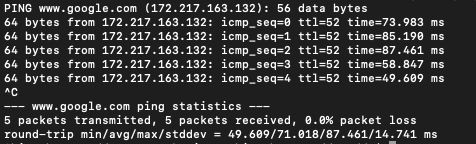
\includegraphics[width=400pt]{Images/image ping.png}
  \caption{Pinging www.google.com}
  \label{fig:2.1}
\end{figure}
\item Using wireshark packet filter ip.addr== host/destination address.
\\eg:- ip.addr == 172.217.163.132
\end{itemize}
\begin{figure}[H]
\centering
  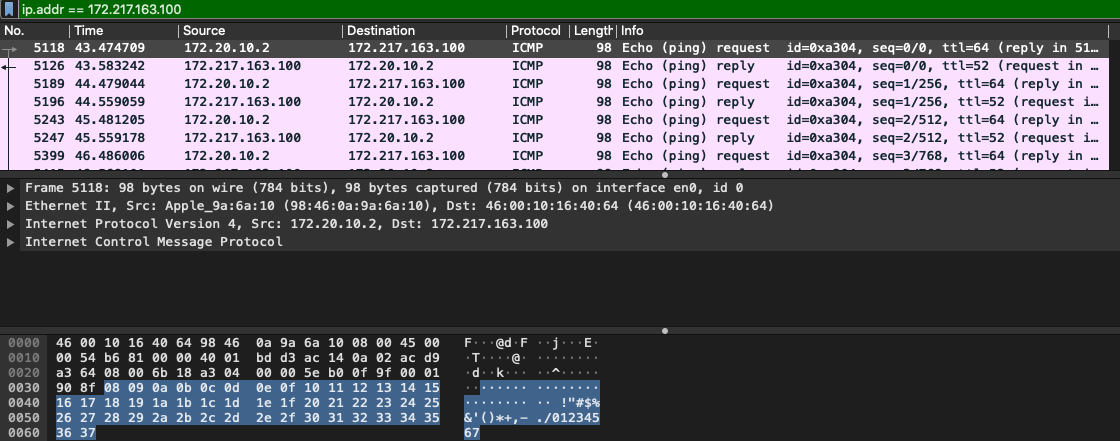
\includegraphics[width=400pt]{Images/DF ping .png}
  \caption{Display filter }
  \label{fig:2.2}
\end{figure}
\section{Packets sent by the host IP Address}
\begin{itemize}
\item The Packets sent by the host when we visit the URL http://www.caid a.org/tools/visualization/mapnet can be displayed with the help of the display filter ip.dst == ip address of the url.
\\eg:- ip.addr == 192.168.43.82.
\begin{figure}[H]
\centering
  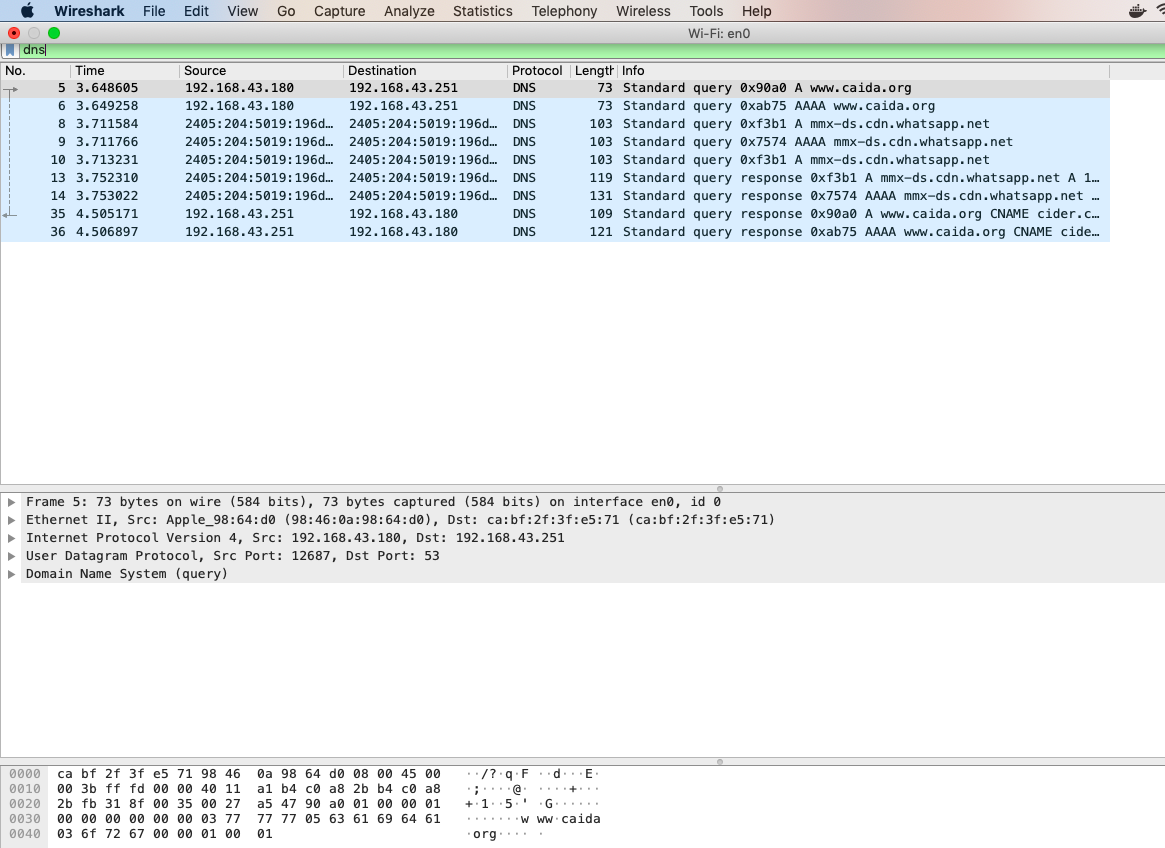
\includegraphics[width=400pt]{Images/host.png}
  \caption{Destination ip Address with DNS filter}
  \label{fig:2.3}
\end{figure}
\end{itemize}
\begin{figure}[H]
\centering
  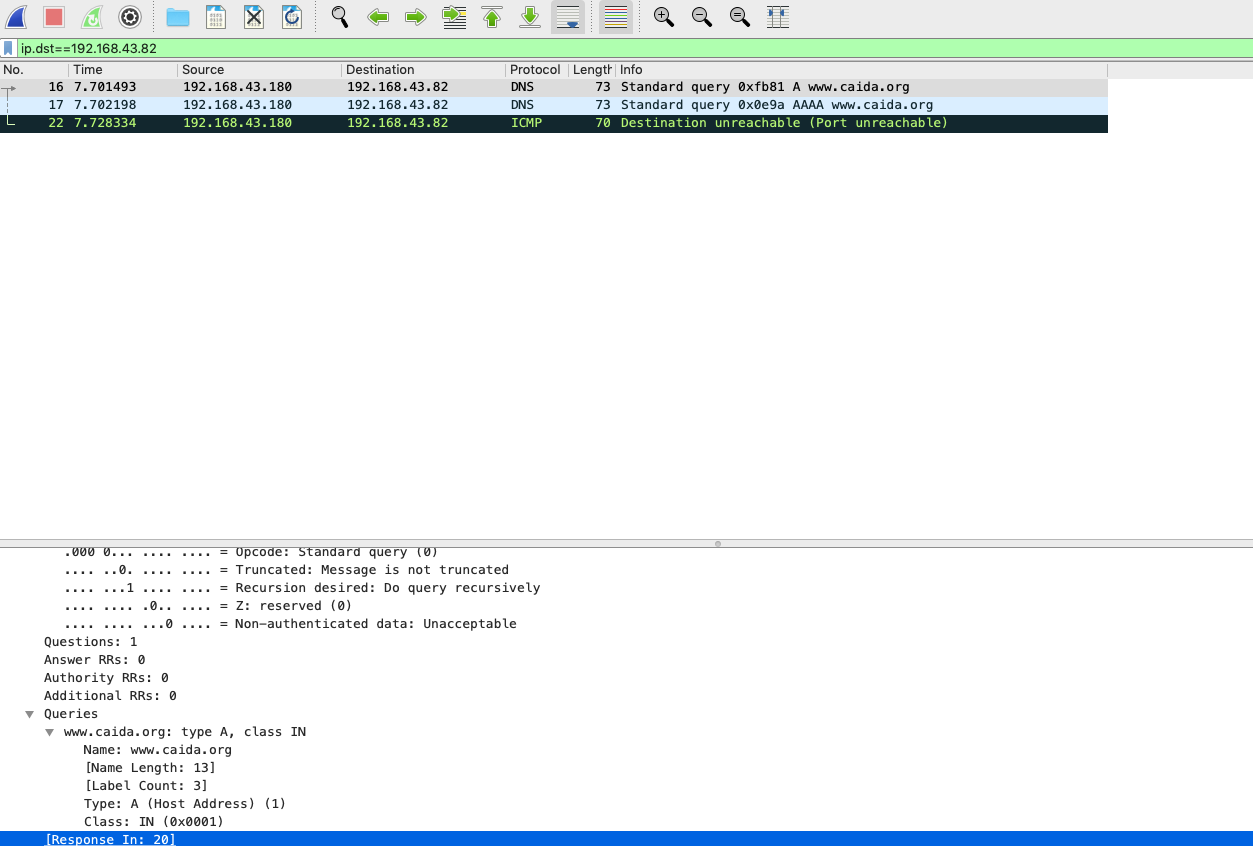
\includegraphics[width=400pt]{Images/new.png}
  \caption{IP address display filter }
  \label{fig:2.4}
\end{figure}
\section{Packets sent by the host MAC Address}
\begin{itemize}
\item The Mac address of my system is 98:46:0a:98:64:d0.
\item The packets sent by the host MAC address, if we visit the URL http://www.caid a.org/tools/visualization/mapnet can be displayed with the filter eth.addr== mac address
\\eg:- eth.addr== 98:46:0a:98:64:d0
\begin{figure}[H]
\centering
  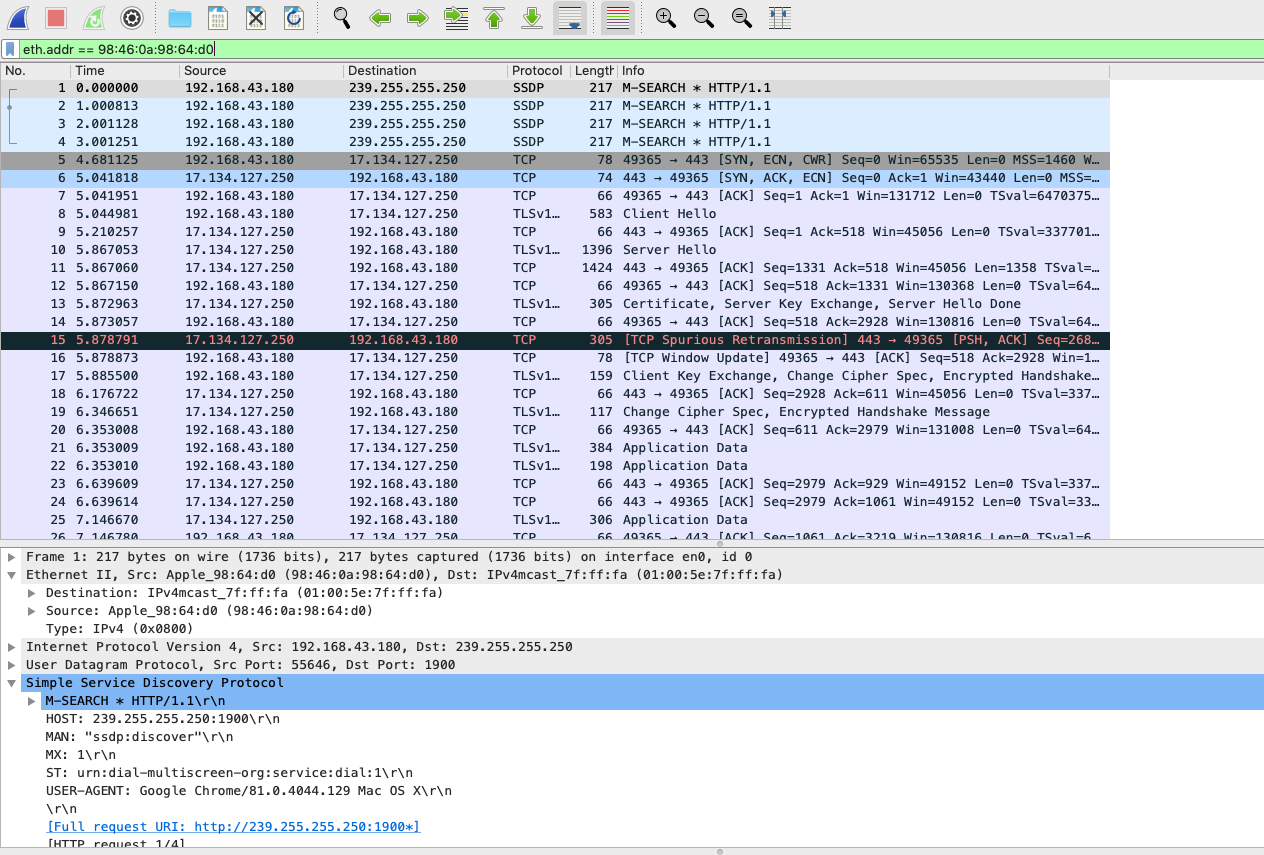
\includegraphics[width=400pt]{Images/mac.png}
  \caption{Mac address display filter}
  \label{fig:2.5}
\end{figure}
\end{itemize}

\section{Difference between MAC and IP address}
\begin{itemize}
\item MAC stands for Media Access Control where as IP stands for Internet Protocol address.
\item The main difference between MAC and IP address is that, MAC Ad- dress indicates the physical address of computer. It uniquely identifies the devices on a network. Where as IP Address is the logical address of the computer is used to uniquely identifies the connection of network with that device in a network.
\item Mac address is a six byte hexa decimal address while ip address is either four(IPV4) byte or six (IPV6)byte address.
\item Mac address operates in the data link layer and ip address operates in the network layer
\end{itemize}

\section{MAC address usage}
 Yes, our system need MAC address for many reasons as below,
\begin{itemize}

\item MAC address is needed for to make a connection to local Ethernet (or wifi) network function. 
\item For a device to communicate with a machine on the LAN (Local Area Network) MAC address is mandatory.
\item Its a low level unique ID for network device.
\item The routers and switches use MAC address tables to find out what devices lie on what ports. This is used to intelligently move packets to the right port. 
\item It’s easier to use MAC address than IP address as a network card can have more then one IP address assigned to it at once, hence it’s more efficient to store the MAC instead.

\end{itemize}

\section{Packets recieved by the host}
\begin{itemize}
\item The packets recieved by the host can be displayed with the display filter: ip.dst=host ip address
\\eg:- ip.dst=92.168.43.180
\begin{figure}[H]
\centering
  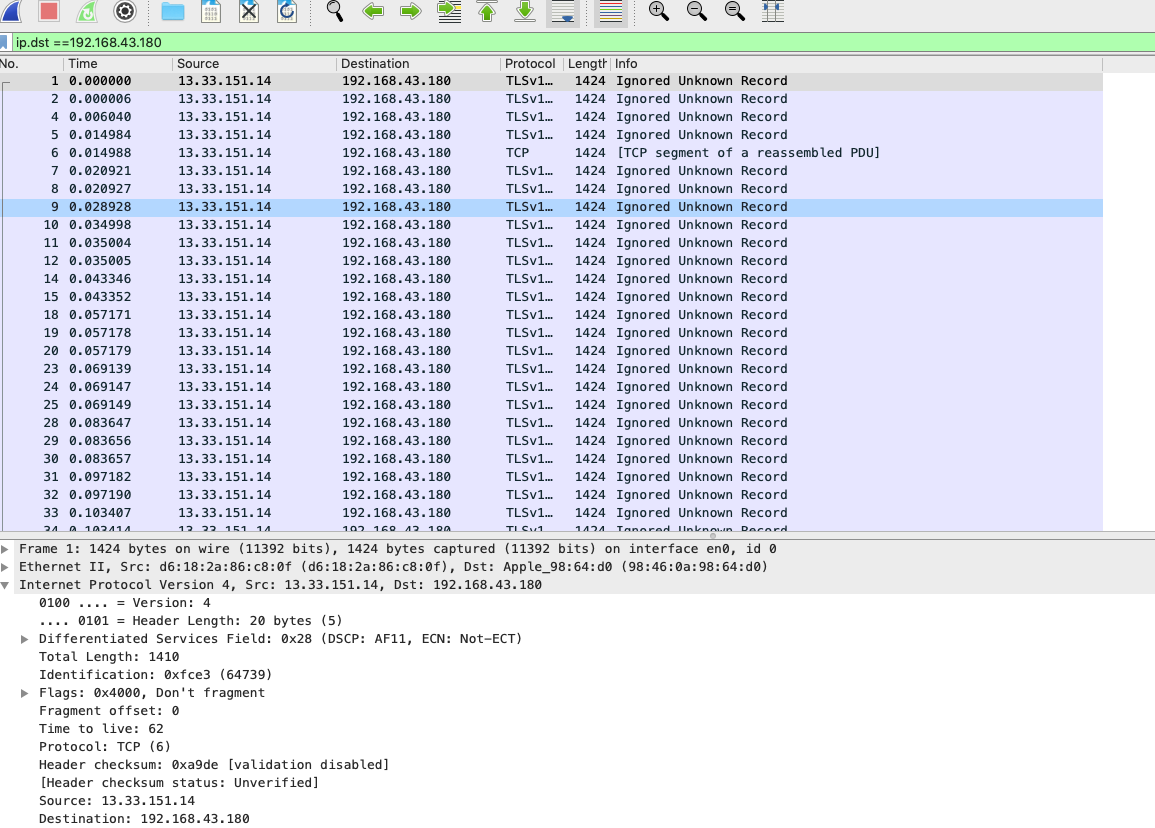
\includegraphics[width=400pt]{Images/ip dst.png}
  \caption{Packets recieved by the host}
  \label{fig:2.6}
\end{figure}
\end{itemize}
\section{Tcp filter to capture packets}
\begin{itemize}
\item Tcp expression that captures packets containing IP datagrams with a source or destination IP address equal to your IP address is as follows:\\

1)host 192.168.43.180.\\

\end{itemize}
\section{Tcp filter to capture packets between 2 hosts}
\begin{itemize}
\item Capture filter expression that captures packets containing IP datagrams between two hosts with IP addresses 10.0.0.3 and 10.0.0.12 both on interface eth0 is as follows
(This is one method, there are other methods)
\\1)host 10.0.0.3 AND host 10.0.0.12
\end{itemize}
\section{TCP Packet Capture}
\begin{itemize}
\item Tcpdump expression that captures TCP packets using port number 22.

1) tcp dst port 22

2) tcp src port 22
\end{itemize}
\section{Display Packets with defined frame size}
\begin{itemize}
\item Syntax for a display filter that shows only IP datagrams with a destination IP address equal to 192.168.178.1 and frame size greater than 350 bytes
\\ip.dst == 192.168.178.1 and frame.len \textgreater 350
\end{itemize}